% This is "sig-alternate.tex" V2.1 April 2013
% This file should be compiled with V2.5 of "sig-alternate.cls" May 2012
%
% This example file demonstrates the use of the 'sig-alternate.cls'
% V2.5 LaTeX2e document class file. It is for those submitting
% articles to ACM Conference Proceedings WHO DO NOT WISH TO
% STRICTLY ADHERE TO THE SIGS (PUBS-BOARD-ENDORSED) STYLE.
% The 'sig-alternate.cls' file will produce a similar-looking,
% albeit, 'tighter' paper resulting in, invariably, fewer pages.
%
% ----------------------------------------------------------------------------------------------------------------
% This .tex file (and associated .cls V2.5) produces:
%       1) The Permission Statement
%       2) The Conference (location) Info information
%       3) The Copyright Line with ACM data
%       4) NO page numbers
%
% as against the acm_proc_article-sp.cls file which
% DOES NOT produce 1) thru' 3) above.
%
% Using 'sig-alternate.cls' you have control, however, from within
% the source .tex file, over both the CopyrightYear
% (defaulted to 200X) and the ACM Copyright Data
% (defaulted to X-XXXXX-XX-X/XX/XX).
% e.g.
% \CopyrightYear{2007} will cause 2007 to appear in the copyright line.
% \crdata{0-12345-67-8/90/12} will cause 0-12345-67-8/90/12 to appear in the copyright line.
%
% ---------------------------------------------------------------------------------------------------------------
% This .tex source is an example which *does* use
% the .bib file (from which the .bbl file % is produced).
% REMEMBER HOWEVER: After having produced the .bbl file,
% and prior to final submission, you *NEED* to 'insert'
% your .bbl file into your source .tex file so as to provide
% ONE 'self-contained' source file.
%
% ================= IF YOU HAVE QUESTIONS =======================
% Questions regarding the SIGS styles, SIGS policies and
% procedures, Conferences etc. should be sent to
% Adrienne Griscti (griscti@acm.org)
%
% Technical questions _only_ to
% Gerald Murray (murray@hq.acm.org)
% ===============================================================
%
% For tracking purposes - this is V2.0 - May 2012

\documentclass{sig-alternate-05-2015}
\usepackage{booktabs}


\begin{document}

% Copyright
%\setcopyright{acmcopyright}
%\setcopyright{acmlicensed}
%\setcopyright{rightsretained}
%\setcopyright{usgov}
%\setcopyright{usgovmixed}
%\setcopyright{cagov}
%\setcopyright{cagovmixed}


% DOI
%\doi{10.475/123_4}

% ISBN
%\isbn{123-4567-24-567/08/06}

%Conference
%\conferenceinfo{PLDI '13}{June 16--19, 2013, Seattle, WA, USA}

%\acmPrice{\$15.00}

%
% --- Author Metadata here ---
%\conferenceinfo{WOODSTOCK}{'97 El Paso, Texas USA}
%\CopyrightYear{2007} % Allows default copyright year (20XX) to be over-ridden - IF NEED BE.
%\crdata{0-12345-67-8/90/01}  % Allows default copyright data (0-89791-88-6/97/05) to be over-ridden - IF NEED BE.
% --- End of Author Metadata ---

%\\TODO:1.tautology prove section 2. set section operation proof 3. function section basic proving onto bijection...
\title{CSCI 3190 \\ Introduction to Discrete Mathematics and Algorithms}
\subtitle{Extended Exercise 3}

\maketitle
\begin{abstract}

\end{abstract}

\keywords{}

\section{Relations and Their Properties}
\begin{enumerate}
\item For each of these relations on the set $\{1, 2, 3, 4\}$, decide
whether it is reflexive, whether it is symmetric, whether
it is antisymmetric, and whether it is transitive.
\begin{enumerate}
\item $\{(2, 2), (2, 3), (2, 4), (3, 2), (3, 3), (3, 4)\}$
\item $\{(1, 1), (1, 2), (2, 1), (2, 2), (3, 3), (4, 4)\}$
\item $\{(2, 4), (4, 2)\}$
\item $\{(1, 2), (2, 3), (3, 4)\}$
\item $\{(1, 1), (2, 2), (3, 3), (4, 4)\}$
\item $\{(1, 3), (1, 4), (2, 3), (2, 4), (3, 1), (3, 4)\}$
\end{enumerate}
\item 
Let $R$ be a relation from a set $A$ to a set $B$. The \textbf{inverse relation}
from $B$ to $A$, denoted by $R^{-1}$, is the set of ordered pairs
$\{(b, a) \mid (a, b) \in R\}$. The \textbf{complementary relation} $\overline{R}$ is the
set of ordered pairs $\{(a, b) \mid (a, b) \notin R\}$.

Let $R$ be the relation $R = \{(a, b) \mid a < b\}$ on the set of
integers. Find
\begin{enumerate}
	\item $R^{-1}$.
	\item $\overline{R}$.
\end{enumerate}
\item Let $R_1 = \{(1, 2), (2, 3), (3, 4)\}$ and $R_2 = \{(1, 1), (1, 2),\\
(2, 1), (2, 2), (2, 3), (3, 1), (3, 2), (3, 3), (3, 4)\}$ be relations
from $\{1, 2, 3\}$ to $\{1, 2, 3, 4\}$. Find
\begin{enumerate}
\item $R_1\cup R_2$. 
\item $R_1 \cap R_2$.
\item $R_1-R_2$. 
\item $R_2-R_1$.
\end{enumerate}
\item Suppose that R and S are reflexive relations on a set A.
Prove or disprove: $R \cap S$ is reflexive.

\item Let $R$ be a symmetric relation. Show that $R^n$ is symmetric for all positive integers $n$. [\textit{Hint:} Since $R$ is symmetric, according to \textbf{Mathematical Induction}, just prove $R^n$ is symmetric when $R^{n - 1}$ is symmetric.]

\item Does a relation on a set $A$, which is symmetric and transitive necessarily
have to be reflexive? Prove it or give a counterexample relation.
\end{enumerate}

\section{Representing Relations}
\begin{enumerate}
\item Represent each of these relationson $\{1, 2, 3\}$ with a matrix (with the elements of this set listed in increasing order).
\begin{enumerate}
	\item $\{(1, 1), (1, 2), (1, 3)\}$ 
	\item $\{(1, 2), (2, 1), (2, 2), (3, 3)\}$
	\item $\{(1, 1), (1, 2), (1, 3), (2, 2), (2, 3), (3, 3)\}$ 
	\item $\{(1, 3), (3, 1)\}$
\end{enumerate}

\item List the ordered pairs in the relations on $\{1, 2, 3\}$ corresponding to these matrices (where the rows and columns
correspond to the integers listed in increasing order).
\begin{enumerate}
	\item $\begin{bmatrix}
		1 & 0 & 1\\
		0 & 1 & 0\\
		1 & 0 & 1
	\end{bmatrix}$
	
	\item $\begin{bmatrix}
		0 & 1 & 0\\
		0 & 1 & 0\\
		0 & 1 & 0
	\end{bmatrix}$
	\item $\begin{bmatrix}
		1 & 1 & 1\\
		1 & 0 & 1\\
		1 & 1 & 1
	\end{bmatrix}$
\end{enumerate}

\item How can the matrix representing a relation $R$ on a set $A$
be used to determine whether the relation is irreflexive?

\item How many nonzero entries does the matrix representing
the relation $R$ on $A = \{1, 2, 3, ..., 100\}$ consisting of the
first 100 positive integers have if $R$ is \begin{enumerate}
	\item $\{(a, b) \mid a > b\}$?
	\item $\{(a, b) \mid a \ne b\}$?
	\item $\{(a, b) \mid a = b + 1\}$?
	\item $\{(a, b) \mid a = 1\}$?
	\item $\{(a, b) \mid ab = 1\}$?
\end{enumerate}

\item How can the matrix for $\bar{R}$, the complement of the
relation $R$, be found from the matrix representing $R$,
when $R$ is a relation on a finite set $A$?

\item Draw the directed graphs representing each of the relations.
\begin{enumerate}
	\item $\{(1, 2), (1, 4), (2, 3), (2, 4), (3, 4)\}$
	\item $\{(1, 1), (1, 4), (2, 2), (3, 3), (4, 1)\}$
	\item $\{(1, 2), (1, 3), (1, 4), (2, 1), (2, 3), (2, 4),\\ (3, 1), (3, 2),
		(3, 4), (4, 1), (4, 2), (4, 3)\}$
	\item $\{(2, 4), (3, 1), (3, 2), (3, 4)\}$
\end{enumerate}

\item List the ordered pairs in the relations represented by the directed graphs.

	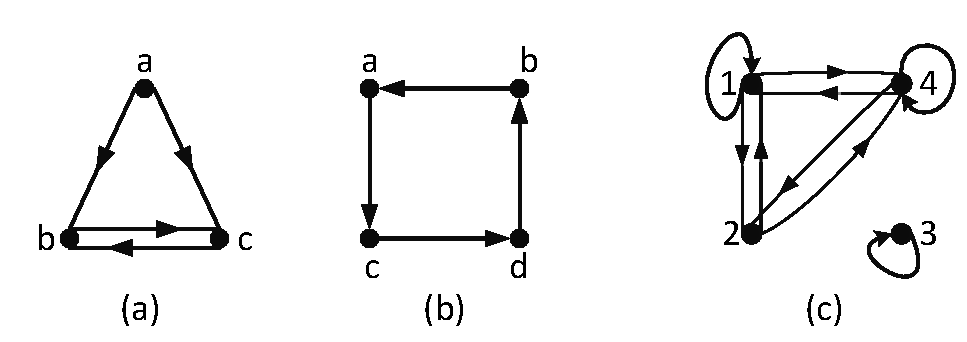
\includegraphics[width=0.4\textwidth]{figs/123.pdf}
\end{enumerate}
\section{Closures of Relations}
\begin{enumerate}
\item Let $R$ be the relation on the set $\{0, 1, 2, 3\}$ containing the ordered pairs $(0, 1), (1, 1), (1, 2), (2, 0), (2, 2)$, and $(3, 0)$. Find the
	\begin{enumerate}
		\item reflexive closure of $R$.
		\item symmetric closure of $R$.
	\end{enumerate}

\item Let $R$ be the relation $\{(a, b) | \text{a divides b}\}$ on the set of
integers. What is the symmetric closure of $R$?
	
\item Find the transitive closures of these relations on $\{1, 2, 3, 4\}$.
	\begin{enumerate}
		\item $\{(1, 2), (2,1), (2,3), (3,4), (4,1)\}$
		\item $\{(2, 1), (2,3), (3,1), (3,4), (4,1), (4, 3)\}$
		\item $\{(1, 2), (1,3), (1,4), (2,3), (2,4), (3, 4)\}$
		\item $\{(1, 1), (1,4), (2,1), (2,3), (3,1), (3, 2), (3,4), (4, 2)\}$
	\end{enumerate}
	
\item Suppose that the relation $R$ on the finite set $A$ is represented by the matrix $M_R$. Show that the matrix that represents the symmetric closure of $R$ is $M_R \vee M^T_R$.

\item When is it possible to define the \textquotedblleft irreflexive closure\textquotedblright\ of a relation $R$, that is, a relation that (a) contains $R$, (b) is irreflexive,
and (c) is contained in every irreflexive relation
that contains $R$?
	
\item Find the smallest relation containing the relation
	
	${(1, 2), (1, 4), (3, 3), (4, 1)}$ that is
	\begin{enumerate}
		\item reflexive and transitive.
		\item symmetric and transitive.
		\item reflexive, symmetric, and transitive.
	\end{enumerate}
	
\item Show that the closure with respect to the property P of
the relation $R = \{(0, 0), (0, 1), (1, 1), (2, 2)\}$ on the set
$\{0, 1, 2\}$ does not exist if P is the property
	\begin{enumerate}
		\item is not reflexive.
		\item has an odd number of elements.
	\end{enumerate}
\end{enumerate}
\section{Equivalence Relations}
\begin{enumerate}
\item Which of these relations on ${0, 1, 2, 3}$ are equivalence
relations? Determine the properties of an equivalence relation
that the others lack.
	\begin{enumerate}
		\item $\{(0, 0), (1, 1), (2, 2), (3, 3)\}$
		\item $\{(0, 0), (0, 2), (2, 0), (2, 2), (2, 3), (3, 2), (3, 3)\}$
		\item $\{(0, 0), (0, 2), (2, 0), (2, 2), (2, 3), (3, 2), (3, 3)\}$
		\item $\{(0, 0), (1, 1), (1, 3), (2, 2), (2, 3), (3, 1), (3, 2),
			(3, 3)\}$
		\item $\{(0, 0), (0, 1), (0, 2), (1, 0), (1, 1), (1, 2), (2, 0),\\
			(2, 2), (3, 3)\}$
	\end{enumerate}
	
\item Suppose that $A$ is a nonempty set, and $f$ is a function that
has $A$ as its domain. Let $R$ be the relation on $A$ consisting
of all ordered pairs $(x, y)$ such that $f (x) = f (y)$.
	\begin{enumerate}
		\item Show that R is an equivalence relation on A.
		\item What are the equivalence classes of R?
	\end{enumerate}
	
\item Show that the relation $R$ consisting of all pairs $(x, y)$ such
that $x$ and $y$ are bit strings of length three or more that
agree in their first three bits is an equivalence relation on
the set of all bit strings of length three or more.

\item Let R be the relation on the set of ordered pairs of positive
integers such that $((a, b), (c, d)) \in R $ if and only if
$a + d = b + c$. Show that $R$ is an equivalence relation.

\item Show that the relation R on the set of all bit strings such
that $s R t$ if and only if $s$ and $t$ contain the same number
of $1$s is an equivalence relation.

\item Find the smallest equivalence relation on the set
$\{a, b, c, d, e\}$ containing the relation $\{(a, b), (a, c),
	(d, e)\}$.

\item Each bead on a bracelet with three beads is either red,
white, or blue, as illustrated in the figure shown.
Define the relation $R$ between bracelets as: $(B_1,B_2)$,
where $B_1$ and $B_2$ are bracelets, belongs to $R$ if and only
if $B_2$ can be obtained from $B_1$ by rotating it or rotating it
and then reflecting it.
\begin{enumerate}
	\item Show that $R$ is an equivalence relation.
	\item What are the equivalence classes of $R$?
\end{enumerate}

\item Do we necessarily get an equivalence relation when we
form the transitive closure of the symmetric closure of
the reflexive closure of a relation?

\item Do we necessarily get an equivalence relation when we
form the symmetric closure of the reflexive closure of the
transitive closure of a relation?

\item Devise an algorithm to find the smallest equivalence relation
containing a given relation.

\end{enumerate}

\section{Partial Orderings}
\begin{enumerate}
\item Which of these relations on $\{0, 1, 2, 3\}$ are partial orderings? Determine the properties of a partial ordering that
the others lack.
	\begin{enumerate}
		\item $\{(0, 0), (1, 1), (2, 2), (3, 3)\}$ 
		\item $\{(0, 0), (1, 1), (2, 0), (2, 2), (2, 3), (3, 2), (3, 3)\}$
		\item $\{(0, 0), (1, 1), (1, 2), (2, 2), (3, 3)\}$
		\item $\{(0, 0), (1, 1), (1, 2), (1, 3), (2, 2), (2, 3), (3, 3)\}$
		\item $\{(0, 0), (0, 1), (0, 2), (1, 0), (1, 1), (1, 2), (2, 0), (2, 2), (3, 3)\}$
	\end{enumerate}

\item Is $(S,R)$ a poset if $S$ is the set of all people in the world
and $(a, b) \in R$, where $a$ and $b$ are people, if
\begin{enumerate}
	\item $a$ is taller than $b$?
	\item $a$ is not taller than $b$?
	\item $a = b$ or $a$ is an ancestor of $b$?
	\item $a$ and $b$ have a common friend?
\end{enumerate}

\item Which of these are posets?
\begin{enumerate}
	\item $(\mathbb{Z}, =)$
	\item $(\mathbb{Z}, \ne)$
	\item $(\mathbb{Z}, \le)$
	\item $(\mathbb{Z}, \nmid)$
\end{enumerate}

\item Determine whether the relations represented by these
zero–one matrices are partial orders.
\begin{enumerate}
	\item 
	$\begin{bmatrix}
		1 & 1 & 1\\
		1 & 1 & 0\\
		0 & 0 & 1
	\end{bmatrix}$
	\item 
	$\begin{bmatrix}
		1 & 1 & 1\\
		0 & 1 & 0\\
		0 & 0 & 1
	\end{bmatrix}$
	\item 
	$\begin{bmatrix}
		1 & 1 & 1 & 0\\
		0 & 1 & 1 & 0\\
		0 & 0 & 1 & 1\\
		1 & 1 & 0 & 1
	\end{bmatrix}$
\end{enumerate}

\item Find two incomparable elements in these posets.
\begin{enumerate}
	\item $(P(\{0, 1, 2\}), \subseteq)$
	\item $(\{1, 2, 4, 6, 8\}, |)$
\end{enumerate}

\item Find the lexicographic ordering of the bit strings 0, 01,
11, 001, 010, 011, 0001, and 0101 based on the ordering
$0 < 1$.

\item Draw the graph representation for the following poset.
	\begin{enumerate}
		\item \textquotedblleft less than or equal to \textquotedblright relation on $\{0, 2, 5, 10, 11, 15\}.$
		\item divisibility on the set $\{1, 2, 3, 6, 12, 24, 36, 48\}$.
	\end{enumerate}

\item Show that lexicographic order is a partial ordering on the
Cartesian product of two posets.

\item Answer these questions for the poset $(\{3, 5, 9, 15,	24, 45\}, \mid)$.
\begin{enumerate}
	\item Find the maximal elements.
	\item Find the minimal elements.
	\item Is there a greatest element?
	\item Is there a least element?
	\item Find all upper bounds of $\{3, 5\}$.
	\item Find the least upper bound of $\{3, 5\}$, if it exists.
	\item Find all lower bounds of $\{15, 45\}$.
	\item Find the greatest lower bound of $\{15, 45\}$, if it exists.
\end{enumerate}

\item 
	\begin{enumerate}
		\item Show that there is exactly one greatest element of a
		poset, if such an element exists.
		\item Show that there is exactly one least element of a poset,
		if such an element exists.
		\item Show that there is exactly one maximal element in a
		poset with a greatest element.
		\item Show that there is exactly one minimal element in a
		poset with a least element.
	\end{enumerate}
\end{enumerate}

\nocite{*}
\bibliographystyle{abbrv}
\bibliography{ref}  % sigproc.bib is the name of the Bibliography in this case
 
\clearpage
%APPENDICES are optional
%\balancecolumns
\appendix
%Appendix A
\section{Answer}

\subsection{Relations and Their Properties}
\begin{enumerate}
\item
\begin{enumerate}
	\item Transitive
	\item Reflexive, symmetric, transitive
	\item Symmetric
	\item Antisymmetric
	\item Reflexive, symmetric, antisymmetric, transitive
	\item None of these properties
\end{enumerate}

\item 
\begin{enumerate}
	\item $R = \{(a, b) \mid a > b\}$.
	\item $R = \{(a, b) \mid a \ge b\}$.
\end{enumerate}

\item
\begin{enumerate}
	\item  $\{(1,2), (2,3), (3,4), (1,1), (2,1), (2,2), (3,1), (3,2), (3,3)\}$
	\item $\{(1,2), (2,3), (3,4)\}$
	\item $\{\emptyset\}$
	\item $\{(1,1), (2,1), (2,2), (3,1), (3,2), (3,3)\}$
\end{enumerate}

\item Proof: $R \cap S$ is reflexive means that $(a,a) \in R\cap S $ for every element $a$ of set $A$.
Since $R$ and $S$ are reflexive, then $(a,a)\in R $ and $(a,a)\in S$ for every element of $A$.
Therefore $(a,a)$ must be in their intersection.

\item Proof by induction:

Basis Step: $R^1= R$ is symmetric is True.

Inductive Step: Assume that $R^n$ is symmetric.

To Prove that $R^{n+1}$ is symmetric.

$R^{n+1}$ is symmetric if for all $(x,y)$ in $R^{n+1}$, we have $(y,x)$ is in $R^{n+1}$ as well.

Assume that $(x,y)$ is in $R^{n+1}$.

Now, $R^{n+1}=R^n\circ R=R\circ R^n$.

We know that if $(x,y)\in R\circ R^n$, then by the definition of composition there
exists a $z$ in $A$ such that $xRz$ and $z(R^n)y$ i.e $(x,z)$ is in $R$ and $(z,y)$ is in $R
^n$ And we also know that $R$ and $R^n$ are symmetric, which implies that $(z,x)$ is
in $R$ and also $(y,z)$ is in $R^n$.

Therefore, by definition of composition, $(y,x)\in R\circ R^n$; i.e. $(y,x)\in R
^{n+1}$.

\item Counter Example Relation:

Let $A=\{a, b, c\}$

Let $R$ be a relation on set $A$

$R =\{(a, a), (b, b), (a, b), (b, a)\}$

This relation is symmetric and transitive but not reflexive since it does not
contain $(c,c)$.

\end{enumerate}

\subsection{Representing Relations}
\begin{enumerate}
\item 
\begin{enumerate}
	\item 
	$\begin{bmatrix}
		1 & 1 & 1\\
		0 & 0 & 0\\
		0 & 0 & 0
	\end{bmatrix}$
	\item 
	$\begin{bmatrix}
	0 & 1 & 0\\
	1 & 1 & 0\\
	0 & 0 & 1
	\end{bmatrix}$
	\item 
	$\begin{bmatrix}
	1 & 1 & 1\\
	0 & 1 & 1\\
	0 & 0 & 1
	\end{bmatrix}$
	\item 
	$\begin{bmatrix}
	0 & 0 & 1\\
	0 & 0 & 0\\
	1 & 0 & 0
	\end{bmatrix}$
\end{enumerate}

\item \begin{enumerate}
	\item (1, 1), (1, 3), (2, 2), (3, 1), (3, 3) 
	\item (1, 2), (2, 2), (3, 2)
	\item (1, 1), (1, 2), (1, 3), (2, 1), (2, 3), (3, 1), (3, 2),
	(3, 3)
\end{enumerate}

\item The relation is irreflexive if and only if the main diagonal of the matrix contains only $0$s.

\item \begin{enumerate}
	\item 4950 
	\item 9900
	\item 99
	\item 100
	\item 1
\end{enumerate}

\item Change each 0
to a 1 and each 1 to a 0.

\item
	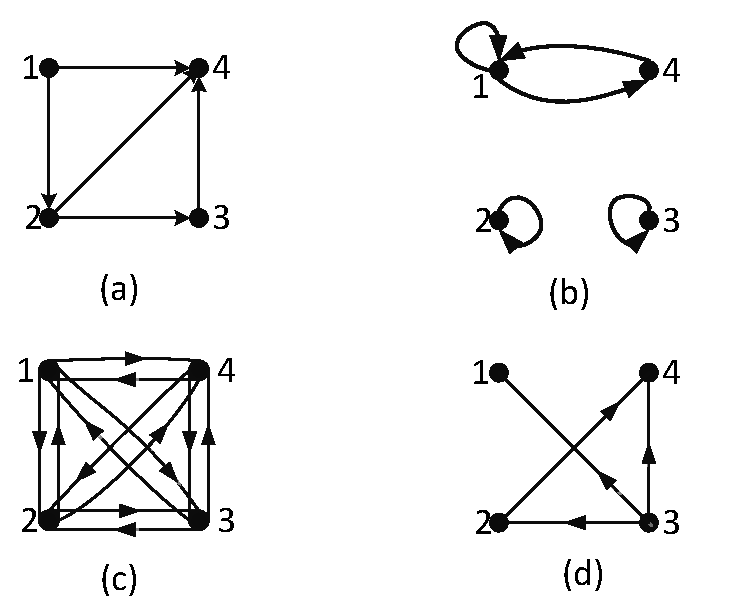
\includegraphics[width=0.5\textwidth]{figs/122.pdf}
	
\item
\begin{enumerate}
	\item $\{(a, b), (a, c), (b, c), (c, b)\}$
	\item $\{(a, c), (b, a), (c, d), (d, b)\}$
	\item $\{(1, 1), (1, 4), (1, 2), (4, 1), (4, 4),\\ (4, 2), (2, 1),
		(2, 4), (3, 3)\}$
\end{enumerate}

\end{enumerate}
\subsection{Closures of Relations}
\begin{enumerate}
\item 
	\begin{enumerate}
		\item $\{(0, 0), (0, 1), (1, 1), (1, 2), (2, 0), (2, 2), (3, 0), (3, 3)\}$
		\item $\{(0, 1), (0, 2), (0, 3), (1, 0), (1, 1), (1, 2), (2, 0), (2, 1),\\
			(2, 2), (3, 0)\}$
	\end{enumerate}

\item
$\{(a, b) | \text{a divides b or b divides a}\}$	

\item
	\begin{enumerate}
		\item 
		$\begin{bmatrix}
		1 & 1 & 1 & 1\\
		1 & 1 & 1 & 1\\
		1 & 1 & 1 & 1\\
		1 & 1 & 1 & 1
		\end{bmatrix}$
		\item
		$\begin{bmatrix}
		0 & 0 & 0 & 0\\
		1 & 0 & 1 & 1\\
		1 & 0 & 1 & 1\\
		1 & 0 & 1 & 1
		\end{bmatrix}$
		\item
		$\begin{bmatrix}
		0 & 1 & 1 & 1\\
		0 & 0 & 1 & 1\\
		0 & 0 & 0 & 1\\
		0 & 0 & 0 & 0
		\end{bmatrix}$
		\item
		$\begin{bmatrix}
		1 & 1 & 1 & 1\\
		1 & 1 & 1 & 1\\
		1 & 1 & 1 & 1\\
		1 & 1 & 1 & 1
		\end{bmatrix}$		
	\end{enumerate}
	
\item The symmetric closure of $R$ is $R \cup R^{-1}$. $M_{R \cup R^{-1}} = M_R \vee M_{R^{-1}} = M_R \vee M_R^T$.

\item Only when $R$ is irreflexive, in which case it is its own closure.

\item
	\begin{enumerate}
		\item $\{(1, 1), (1, 2),
			(1, 4), (2, 2), (3, 3), (4, 1), (4, 2), (4, 4)\}$
		\item $\{(1, 1),(1, 2), (1, 4), (2, 1), (2, 2), (2, 4),\\ (3, 3), (4, 1), (4, 2),
			(4, 4)\}$
		\item $\{(1, 1), (1, 2), (1, 4), (2, 1), (2, 2), (2, 4),\\ (3, 3),
			(4, 1), (4, 2), (4, 4)\}$
	\end{enumerate}

\item 
	\begin{enumerate}
		\item Because $R$ is reflexive, every
		relation containing it must also be reflexive.
		\item Both $\{(0, 0),
			(0, 1), (0, 2), (1, 1), (2, 2)\}$ and $\{(0, 0),\\ (0, 1), (1, 0), (1, 1),
			(2, 2)\}$ contain R and have an odd number of elements, but
		neither is a subset of the other.
	\end{enumerate}
\end{enumerate}
\subsection{Equivalence Relations}
\begin{enumerate}
\item
	\begin{enumerate}
		\item Equivalence relation \item Not reflexive, not transitive
		\item Equivalence relation \item Not transitive \item Not symmetric,
		not transitive
	\end{enumerate}
\item
	\begin{enumerate}
		\item  $(x, x) \in R $ because $f (x) = f (x)$. Hence, $R$ is reflexive.
		
		$(x, y) \in R$ if and only if $f (x) = f (y)$, which holds if and
		only if $f (y) = f (x)$ if and only if $(y, x) \in R.$ Hence, R is
		symmetric. 
		
		If $(x, y) \in R$ and $(y, z) \in R,$ then $f (x) = f (y)$
		and $f (y) = f (z)$. Hence, $f (x) = f (z)$. Thus,$ (x, z) \in R$.
		It follows that $R$ is transitive. 
		\item   The sets $f^{-1}(b)$ for $b$ in the range of $f$.
	\end{enumerate}

\item 
Let $x$ be a bit string of length 3 or more.

Because $x$ agrees with itself in the first three bits, $(x, x)\in R.$
Hence, $R$ is reflexive. 

Suppose that $(x, y) \in R.$ Then $x$ and $y$ agree in the first three bits. 
Hence, $y$ and $x$ agree in the first three bits. Thus, $(y, x)\in R$. $R$ is symmetric.

If $(x, y)$ and $(y, z)$ are in $R$, then
$x$ and $y$ agree in the first three bits, as do $y$ and $z$. Hence, $x$
and $z$ agree in the first three bits. Hence, $(x, z) \in R.$ It follows
that $R$ is transitive.

\item
For reflexivity,
$((a, b), (a, b))\in R$ because $a +b = b +a$. For symmetry, if
$((a, b), (c, d))\in R,$ then $a + d = b + c$, so $c + b = d + a$,
so $((c, d), (a, b))\in R.$ For transitivity, if $((a, b), (c, d)) \in R$
 and $((c, d), (e, f )) \in R,$ then $a+d = b+c$ and $c+e = d+f$ ,
so $a + d + c + e = b + c + d + f$ , so $a + e = b + f $,
so $((a, b), (e, f ))\in R.$ 

\item $R$ is reflexive because a bit string $s$ has the same 
number of $1$s as itself. 

$R$ is symmetric because
$s$ and $t$ having the same number of $1$s implies that $t$ and $s$ do.

$R$ is transitive because $s$ and $t$ having the same number of $1$s,
and $t$ and $u$ having the same number of $1$s implies that $s$ and
$u$ have the same number of $1$s.

\item $\{(a, a), (a, b),
	(a, c), (b, a), (b, b), (b, c), (c, a),\\ (c, b), (c, c), (d, d), (d, e),
	(e, d), (e, e)\}$

\item 
\begin{enumerate}
	\item $R$ is
	reflexive because any coloring can be obtained from itself via
	a 360-degree rotation. To see that $R$ is symmetric and transitive,
	use the fact that each rotation is the composition of two reflections and conversely the composition of two reflections
	is a rotation. Hence, $(B_1, B_2)$ belongs to $R$ if and only
	if $B_2$ can be obtained from $B_1$ by a composition of reflections.
	So if $(B_1, B_2)$ belongs to $R$, so does $(B_2, B_1)$ because
	the inverse of the composition of reflections is also a composition
	of reflections (in the opposite order). Hence, $R$ is
	symmetric. To see that $R$ is transitive, suppose $(B_1, B_2)$ and
	$(B_2, B_3)$ belong to $R$. Taking the composition of the reflections
	in each case yields a composition of reflections, showing
	that $(B_1,B_3)$ belongs to $R$. 
	\item We express colorings with sequences
	of length four, with $r$, $w$ and $b$ denoting red, white and blue,
	respectively. We list letters denoting the colors of the upper
	ball, right ball, and left ball, in that order. The equivalence classes are: $\{rrr\}$, $\{www\}$, $\{bbb\}$, $\{rrw, rwr, wrr\}$, $\{rrb, rbr, brr\}$, $\{wwr, wrw, rww\}$, $\{wwb, wbw, bww\}$, $\{bbr, brb, rbb\}$, $\{bbw, bwb, wbb\}$.
\end{enumerate}

\item Yes.

\item Yes.

\item First form the reflexive closure of $R$, then form
the symmetric closure of the reflexive closure, and finally
form the transitive closure of the symmetric closure of the
reflexive closure.
\end{enumerate}

\subsection{Partial Orderings}
\begin{enumerate}
\item 
\begin{enumerate}
	\item Is a partial ordering.
	\item Not antisymmetric, not transitive.
	\item Is a partial ordering.
	\item Is a partial ordering.
	\item Not antisymmetric, not transitive.
\end{enumerate}

\item 
\begin{enumerate}
	\item No.
	\item Yes.
	\item Yes.
	\item No.
\end{enumerate}

\item 
\begin{enumerate}
	\item Yes.
	\item No.
	\item Yes.
	\item No.
\end{enumerate}

\item 
\begin{enumerate}
	\item No.
	\item Yes.
	\item No.
\end{enumerate}

\item 
\begin{enumerate}
	\item $\{0\}$ and $\{1\}$, for instance.
	\item 4 and 6, for instance.
\end{enumerate}

\item $0 < 0001 < 001 < 01 < 010 < 0101 < 011 < 11$.

\item 
	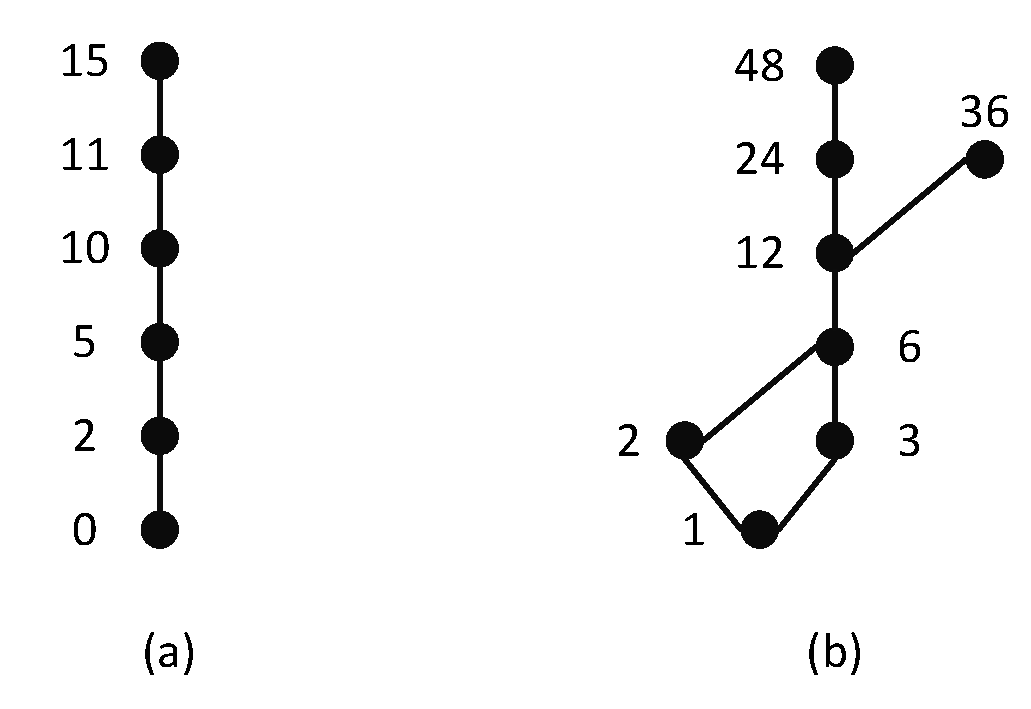
\includegraphics[width=0.4\textwidth]{figs/252.pdf}
	
\item 
Because $(a, b)\preceq (a, b)$, $\preceq$ is reflexive. 

If$(a1, a2)\preceq (b1, b2)$ and $(a1, a2)\neq (b1, b2)$, either $a1\prec b1$, or
$a1 = b1$ and $a2 \prec b2$. In either case, $(b1, b2)$ is not less than or
equal to $(a1, a2)$. Hence, $\preceq$ is antisymmetric. 

Suppose that
$(a1, a2)\prec (b1, b2) \prec (c1, c2)$. Then if $a1\prec b1$ or $b1\prec c1$,
we have $a1 \prec c1$, so $(a1, a2) \prec (c1, c2)$, but if $a1 = b1 = c1$,
then $a2 \prec b2 \prec c2$, which implies that $(a1, a2) \prec (c1, c2)$.
Hence, $\preceq$ is transitive.

\item
\begin{enumerate}
	\item 24, 45 
	\item 3, 5
	\item No
	\item No
	\item 15, 45
	\item 15
	\item 15, 5, 3
	\item 15
\end{enumerate}

\item
	\begin{enumerate}
		\item Suppose that there are two different elements $x$ and $y$ that are greatest.
		
		So $\forall a \in S$ and $a\preceq x$. 
		
		Also, $\forall a \in S$ and $a\preceq y$. 
		
		Since $x \in S$ and $y\in S$, we have $x\preceq y$ and also $y \preceq x$. 
		
		So $x=y$ because relation $\preceq$ is antisymmetric.
		
		Which is a contradiction because we started out with $x$ and $y$ being different
		elements. So there canot be two different elements that are greatest. So if
		exists then there is only a unique element that is greatest.

		\item Suppose that there are two different elements $x$ and $y$ that are least.
		
		So $\forall a \in S$ and $x\preceq a$. 
		
		Also, $\forall a \in S$ and $y\preceq a$. 
		
		Since $x \in S$ and $y\in S$, we have $x\preceq y$ and also $y \preceq x$. 
		
		So $x=y$ because relation $\preceq$ is antisymmetric.
		
		Which is a contradiction because we started out with $x$ and $y$ being different
		elements. So there canot be two different elements that are least. So if
		exists then there is only a unique element that is least.
		
		\item Suppose that $x$ is maximal and that $y$ is the largest
		element. Then $x \preceq y$. Because $x$ is not less than $y$, it follows
		that $x = y$. By (a) $y$ is unique. Hence, $x$ is
		unique.
		\item Suppose that $x$ is minimal and that $y$ is the smallest
		element. Then $x \preceq y$. Because $x$ is not greater than $y$, it follows
		 that $x = y$. By (b) $y$ is unique. Hence, $x$ is unique.
	\end{enumerate}
\end{enumerate}
\end{document}
